\documentclass[conference]{IEEEtran}

\usepackage[english]{babel}
\usepackage{amsmath}
\usepackage{amsfonts}
\usepackage{amssymb}
\usepackage{amsthm}
\usepackage{epsfig}
\usepackage{epstopdf} % pdflatex -synctex=1 -interaction=nonstopmode -shell-escape %.tex

\newcommand{\preferal}[1]{\underset{#1}{\succ}}
\newcommand{\equivalent}[1]{\underset{#1}{\sim}}
\newcommand{\argmax}{\operatorname*{arg\,max}}
\newcommand{\argmin}{\operatorname*{arg\,min}}

\newtheorem{definition}{Definition}
\newtheorem{theorem}{Theorem}


\usepackage{fmtcount}
\usepackage{graphicx}
\usepackage{courier}

\graphicspath{{Figures/}{img/}}

\usepackage[colorlinks=true, citecolor=Red, urlcolor=blue, pdfhighlight =/O]{hyperref}
%\hypersetup{
% colorlinks=false,
% citecolor=Violet,
% linkcolor=Red,
% urlcolor=Blue}


\usepackage[usenames,dvipsnames]{pstricks}
\usepackage{epsfig}
\usepackage{pst-grad} % For gradients
\usepackage{pst-plot} % For axes

% correct bad hyphenation here
\hyphenation{op-tical net-works semi-conduc-tor}

\usepackage[acronym,toc]{glossaries}
\newacronym{NAC}{NAC}{Network Average Consensus}


\begin{document}
%
% paper title
% can use linebreaks \\ within to get better formatting as desired
\title{Multi-Preferential Consensus Parameters Selection for Cognitive Radio}


% author names and affiliations
% use a multiple column layout for up to three different
% affiliations

\author{
\IEEEauthorblockN{
 Clément Duhart$^{\ddagger}$, Rafik Zitouni$^{\ddagger}$ $^{\dagger}$ and Laurent George$^{\ddagger}$ $^{\dagger}$
}
\IEEEauthorblockA{
$^{\ddagger}$ ECE Paris-LACSC Laboratory \\
37 Quai de Grenelle, 75015, Paris, France\\
$^{\dagger}$ LISSI / UPEC \\
120, rue Paul Armangot\\
94400 Vitry S/Seine, France\\
Email: \{zitouni, ataman, mathian, lgeorge\}@ece.fr\\}
}



% use for special paper notices
%\IEEEspecialpapernotice{(Invited Paper)}




% make the title area
\maketitle



\begin{abstract}
%\boldmath
TODO 
\end{abstract}

\begin{IEEEkeywords}
Cognitive Radio, adaptive modulation, Wireless networks, consensus.
\end{IEEEkeywords}


\section{INTRODUCTION}
TODO\\

Recently, the number of the wireless networks applications increases in the same frequency band. The coexistence of multiple wireless transmission technologies leads to degrade their performances. The reciprocal influence is avoided by sharing this resource without prior knowledge. The cognitive radio network proposes to exploit opportunistically the underused electromagnetic spectrum. 

The spectrum access is a significant problem because it depend on the legislation defined by different institutions (e.g FCC: Federal Communications Commission) \cite{Haykin2005}. The spectrum licensed is occupied principally by the primary user. The frequency holes appear at particular periods of time and specific geographic location when the licensed frequency band is free and not used by that user. The utilization can be improved by allowing to the secondary user a temporarily occupation of the spectrum holes. The Dynamic Spectrum Access (DSA) networks is the secondary opportunistic user of the spectrum without interfering with the primary user \cite{Liu2011}. The cognitive radio with an efficient DSA is implemented on the reconfigurable Software Defined Radio (SDR) \cite{Mitola1993}. The optimal performances of the secondary user is obtained by the capability to adapt to the surrounding environment. This environment is characterized by the sensed informations, such as transmission frequency, bandwidth, number of nodes, noise power, modulation, etc \cite{Liu2011}. 



Adaptive modulation and channel to improve data rate. \\

Nodes consensus for wireless transmission improvement.\\

Contribution and related work. \\

\section{RELATED WORKS}


TODO

\section{SYSTEM MODEL}
The purpose of our work is to achieve a hight data rate or spectrum efficiency in the cognitive network with a selection of the appropriates parameters or settings. The aggregation of this parameters gives the utility function which is defined to carry out a balance between the power transmission, the modulation type and the channel quality with existence of primary and secondary users.

\subsection{PARAMETER DEFINITION}
We start our system model by the mathematical definition of the transmission parameters. The first parameter is the expression of the Signal Interference Noise Ratio (SINR) in terms of the power transmission, the gain and the thermal noise. Let \textit{N} denotes a set of cochannel labelled  by the integers $i=1,2 \cdots,N$. Where $G_{ij}$ defines the path gain from node $j$ to node $i$. $P_{i}$ indicates the transmission power of node $i$. The signal is represented when $i=j$, otherwise, this is interference. The SINR of node $i$, $\gamma_{i}$ is given by :
 
\begin{equation}
\label{eq-sinr}
\gamma_{i}(P_{i})=\frac{G_{ii}P_{i}}{\underset{j\neq i}{\sum}G_{ij}P_{j}+n_{i}}
\end{equation}

\[
\gamma_{i}(P_{i})=\frac{G_{ii}P_{i}}{I_{i}}
\]

The value of $n_{i}$ denotes the receiver thermal noise power. The total interference and thermal noise are gathered in $I_{i}$.\\

The channel capacity  $C_{i}$ is modelled as function of the frequency bandwidth $\omega_{i}$ and  $\gamma_{i}(P_{i})$   \cite{Shannon1948}. 
%\begin{equation}
%\label{eq-capacity_shannon}
\[
C_{i}=\intop_{0}^{\infty}
 \omega_{i}\log_{2}(1+\gamma_{i}(P_{i}))Pr(\gamma_{i})d
 \gamma_{i}(P_{i})
\]
% \end{equation}

Also, the capacity can be expressed as function of the adjusted transmit power $P_{i}(\gamma_{i})$ to the fading channel \cite{Goldsmith1997}.The parameter $P_{i}(\gamma_{i})$ is the adaptive power relative to $\gamma_{i}$, subject to the average power constraint $\overline{P_{i}}$.
\begin{align}
%\begin{equation}
\label{eq-capacity_Goldsmith}
C_{i}=\underset{\int P_{i}(\gamma_{i})Pr(\gamma_{i})d\gamma_{i}=\bar{P_{i}}}{\max}\intop_{0}^{\infty}\omega_{i}\log_{2}\left(1+\frac{P_{i}(\gamma_{i})\gamma_{i}}{\overline{P_{i}}}\right)\\
Pr(\gamma_{i})d\gamma_{i}(P_{i}) \nonumber
%\end{equation}
\end{align}
 
To maximize the channel capacity in (\ref{eq-capacity_Goldsmith}), the transmit power adaptation is given as follows : 
\begin{equation}
\label{Power_noise}
\frac{P_{i}(\gamma_{i})}{\overline{\gamma_{i}}}=\begin{cases}
\frac{1}{\gamma_{i}^{0}(P_{i})}-\frac{1}{\gamma_{i}(P_{i})} & ,\gamma_{i}(P_{i})\geqslant\gamma_{i}^{0}(P_{i})\\
0 & ,\gamma_{i}(P_{i})<\gamma_{i}^{0}(P_{i})
\end{cases}
\end{equation}
Where $\gamma_{i}^{0}(P_{i})$ is some "cutoff" value, when  $\gamma_{i}^{t}(P_{i})
 <\gamma_{i}^{0}(P_{i})$ at time $t$, then no power is allocated to the $i$th channel. The variation of $\gamma(P_{i})$ in the time depend on the probability distribution $Pr$. In the case of the favorable channel more power is allocated for transmission. In contrast, less power will be transmitted. The channel is not used if the value of $\gamma_{i}(P_{i})$ drops down below $\gamma_{0}(P_{i})$.
 
The number of bits transmitted within each symbol is restricted to a finite number of values. With $M$-QAM The constellation size is restricted to $M=2^{j}, j=1,2,...,J$, making the bits per symbol equal to one of a small set of values. The data rate of one channel is defined as the number of bits that can be successfully received within each transmitted symbol. However, the Bit Error Rate $BER$ affect the data rate and it can be approximated for each specific modulation (e.g MPSK, $M$-QAM) \cite{Cheng2008}. We restrict our work to MQAM signal constellations. For fixed $M$ value and symbol period $T$, the data rate $R$ of MQAM modulation \cite{Goldsmith1998} family is equal to:

\[R=[\log_{2}M_{j}-1]/T
\]

On the other hand, the $BER$ is given by the expression \cite{Goldsmith1997} :
\begin{equation}
\label{eq-BER}
BER\approx0.2\exp\left[\frac{-1.5\gamma}{(M-1)}\frac{P_{i}(\gamma)}{\overline{P_{i}}}\right]
\end{equation}
 

To maintain a fixed $BER$, in the equation \ref{eq-BER}, we can adjust $M$ and $P_{i}(\gamma)$

The adaptive modulation is used to maintain a constant $BER$ and to increase the spectral efficiency when wireless channel quality changes. From the expression \ref{eq-BER}, the constellation size is expressed in terms of  $\gamma_{i}$ fade level and the transmit power $P_{i}$ adapted to the interference. 

\begin{equation}
\label{eq-M}
M(\gamma_{i})=1+\frac{1.5\gamma_{i}(P_{i})}{-\ln(5BER)}
 \frac{P_{i}(\gamma_{i})}{\overline{P_{i}}}
\end{equation}

The spectral efficiency is defined as the bit rate per unit hertz (bis/s/Hz), as follow. 
\begin{equation}
\label{efficiency}
E_{i} = C_{i}/\omega_{i}
\end{equation}


The maximum spectral efficiency average is obtained by transmitting at hight data rate when channel conditions are favorable and low data rate when the channel degrades. 
 
\subsection{PARAMETER INTERACTION}
 
\begin{figure}[h]
   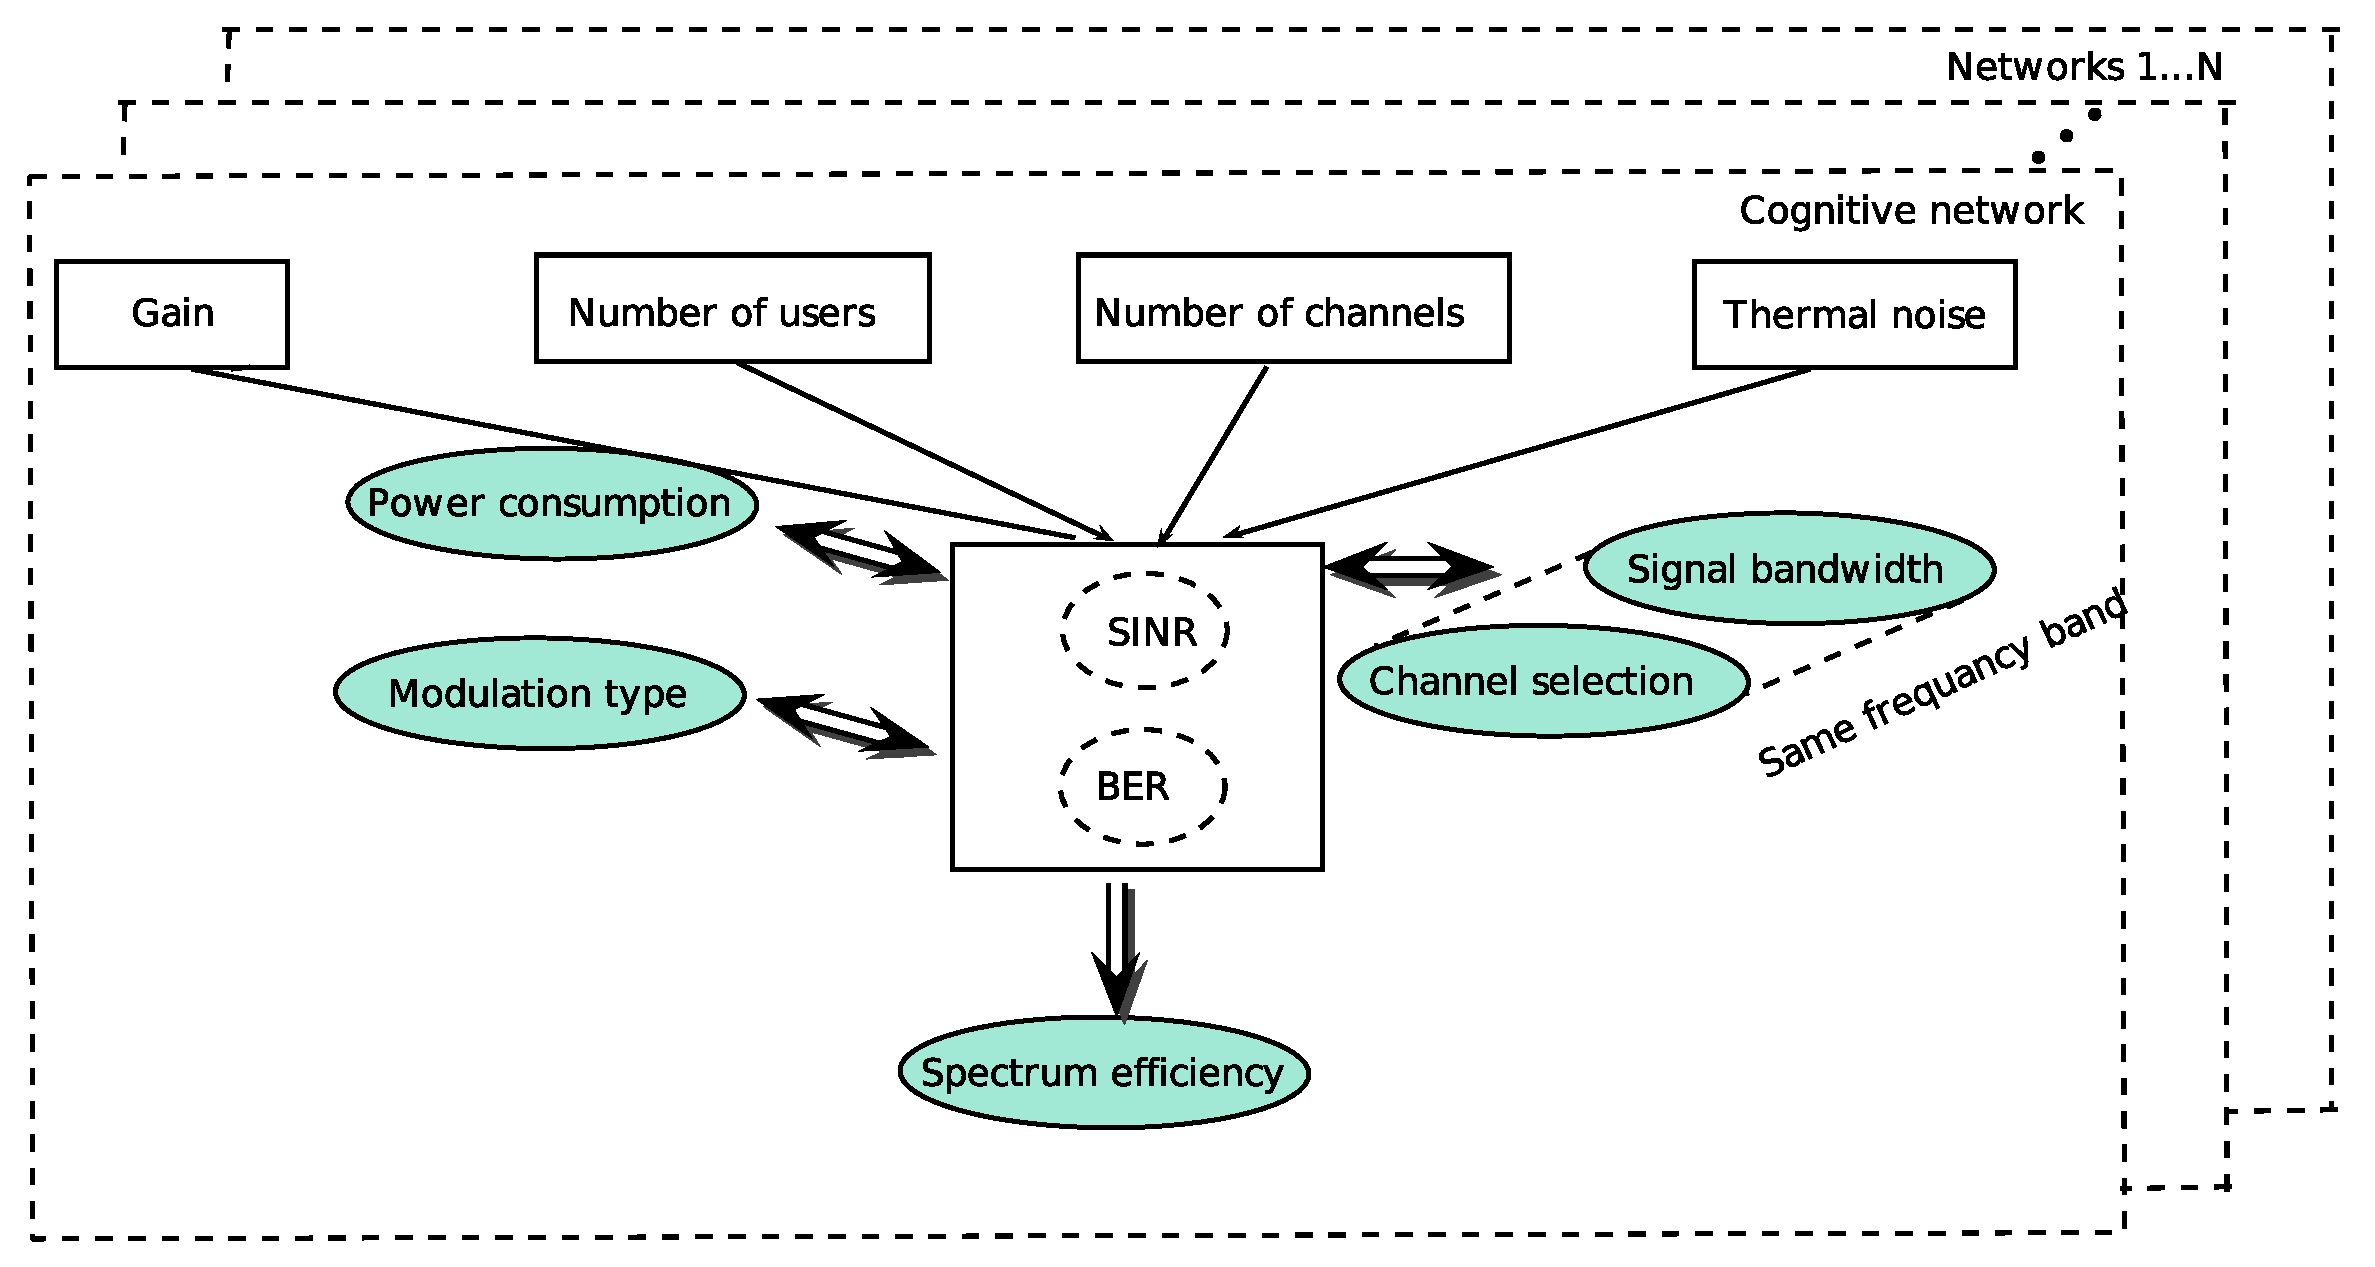
\includegraphics[width=9cm]{fig-1bis.eps}\\
   \caption{Parameter interaction} \label{fig-1}
\end{figure}
 
The schema shown in the Figure \ref{fig-1} presents the $n$ possible networks sharing the same frequency band on the number of the channels. One network is cognitive with adaptive setting and the other networks are fixed and defined by the standard specifications. The schematic rectangles and circles contain respectively the fixed and dynamic parameters, while the arcs are the influence relationships among each other. 

The number of channels is defined for each network in the PHY specifications (e.g IEEE 802.15.4 and IEEE 802.11 have respectively 16 channels and 13 channels in the ISM frequency band). The number of nodes in the network is fixed for period of time. The high gain allows the transmitter to increase the signal strength and permits the receiver to capture the more signal. The thermal noise is approximately white and nearly constant throughout the frequency spectrum. Each channel is defined by the available spectrum or a signal bandwidth. All these environmental and physical parameters affect the SINR and the BER transmission characteristic. 

The spectrum efficiency $E_{i}$ is improved by taking in consideration the signal bandwidth $\omega_{i}$ and the channel capacity $C_{i}$, since it is defined as the report between the channel capacity and signal bandwidth. In the formula (\ref{eq-capacity_Goldsmith}), the channel capacity increase at the same time as the power transmission $P_{i}(\gamma_{i})$ adapted to the noise distribution $Pr(\gamma_{i})$. The power consumption can be minimised with the adapted modulation type. The power transmission and channel selection can be adjusted interactively according to the SINR. The measurement of BER and SINR depend on the settings interactions. However, the objective of the parameters settings is to find a tradeoff between the power consumption, the signal bandwidth or channel selection to achieve the spectrum efficiency.

\subsection{PARAMETER AGGREGATION}
The nodes in the cognitive radio network are the cognitive agent with different profiles. The parameters to choose by the agents are the transmission power, the modulation type and the number of channel. The one to one profile is the communication conditions between neighbouring nodes in one hop transmission. Two nodes should have the same modulation type and channel number to communicate. The Automatic Repeat Request (ARQ) transmission protocol is used to insure the neighbouring synchronisation use of these parameters. The individual nodes setting is the power consumption, which can be controlled without coordination. 
   
To insure a hight spectrum efficiency with tradeoff 

\section{CONSENSUS ALGORITHM}
TODO : Global view \\

\subsection{CR network preferences}
Network of cognitive radio agents $n_i$ is defined with topology G = (V,E) in which each agent only communicates with its neighboring agents $\Upsilon_i = \{j \in V : \{i,j\} \in E\}$ which are inside a range of radius R. Each cognitive radio agents can communicate through several communication profiles $\rho_0, \rho_1 ... \rho_M$ composed of available bandwidth, channel number, etc.

\paragraph*{Communication profile definition  : Add $\rho_j$ definition !}[TODO - Rafik] \\

A profile preference preorder is representative of all node $i$ if for all of them, this preorder is established. Profile preferential preorder of CR communication profile is modelled by Von-Neumann preferential utility [REF].  Metric value of preference preoder is modelled through an inequality of utility function $u^i$ such as in eq \ref{eq-preferential-utility-def}.  

\begin{equation}
\label{eq-preferential-utility-def}
\displaystyle
\forall k, \rho_j \succ \rho_k \Longleftrightarrow \forall i,k,  \rho_j \preferal{i} \rho_k \Longleftrightarrow \forall k, u_j > u_k
\end{equation}

TODO : OWA et PARETO\\

Based on this definition, node preference preorder must evolved to converge to an aggregated preference preorder which is representative of the set of node preference preorder to verify definition given in eq \ref{eq-preferential-utility-def}. In this paper, the aggregation operator studied is the profile utility average through distributed network average consensus.

\subsection{Distributed utility aggregation}
Average consensus of preferences is composed of $M$ average consensus problems to determine a representative utility value for each profile $\rho$ to produce an order of profile utility for all CR network by a distributed way. Distributed network consensus problems is solved asymptotically by using gradient-descent algorithm in which $\dot{u_j}$ are the final average consensus value of initial utility of node $i$ for profile $j$ as summarize in eq \ref{eq-consensus-def} (more details about network average consensus can be found in \cite{Ren2005}). 

\begin{equation}
\label{eq-consensus-def}
\displaystyle
\dot{u_j} =  \lim_{t \to +\infty } u_j(t)  =  {1 \over N } \sum_{i=0}^N u_j^i(0)  \Longleftrightarrow \forall i,j || \dot{u}_j - \dot{u}_j^i || < \varepsilon
\end{equation}

The iterative algorithm of distributed average network consensus is given in eq \ref{eq-consensus-analytic} with its analytic form and in eq \ref{eq-consensus-matrix} with its matrix form and the necessary condition of convergence : $\forall i, W^i < \frac{1}{\Delta}$ with $\Delta = max(\#\Upsilon_i)$.

\begin{equation}
\label{eq-consensus-analytic}
\displaystyle
u_j^i(t+1) = u_j^i(t) - w^i \sum_{k=0}^N[u_j^i(t) - u_j^k(t)]
\end{equation}

\begin{equation}
\label{eq-consensus-matrix}
\displaystyle
U_j(t+1) = [I-WL]U_j(t)
\end{equation}

with L the Laplacian of network G defined in eq \ref{eq-consensus-laplacian} in which A is adjacency matrix of graph G and D a diagonal matrix defined as $L_{i,i} = \#\Upsilon_i$ .

\begin{equation}
\label{eq-consensus-laplacian}
L = D - A = \left\{
      \begin{aligned}
      L_{i,i} &= &\#\Upsilon_i\hspace{2.6cm}\\
      L_{i,j} &= &\left\{
                \begin{aligned}
                -1 \hspace{0.5cm} &if& j \in \Upsilon_i \\
                 0 \hspace{0.5cm} &else& \\
                \end{aligned}
                \right.
      \end{aligned}
    \right.
\end{equation}

By applying network average consensus for each profile preference, each node obtains the same set of average profile aggregated preference utility according to interval error $]- \varepsilon + \dot{u} ; \dot{u} + \varepsilon [$ produced by asymptotic convergence.

\subsection{Robust uniqueness decisions}
Decision rules allows nodes to choice between profiles according to the aggregated utility of profile preferences estimated by previously presented network average consensus. Nodes must make the same choice and so, decision rules have to be strongly discriminant as defined in eq \ref{eq-decision-discriminant} to allow decisions to be uniqueness. 

\begin{theorem}
\label{th-preference}
If only if it exists a profile utility $\dot{u}_j^i$ greater than any other profile utility $\dot{u}_k^i$ for any decision makers $i$ estimated by network average consensus, so that it's ideal average utility value $\dot{u}_j$ is spaced more than $2 \varepsilon$ from any other ideal average utility value $\dot{u}_k $ then this profile is preferred to any other profile by all decision makers. 
 
\begin{equation}
\label{eq-decision-discriminant}
\forall i, k, \exists j / \dot{u}_j^i > \dot{u}_k^i \ \& \ || \dot{u}_j - \dot{u}_k|| > 2 \varepsilon \Longleftrightarrow \rho = \rho^i = j
\end{equation}

\end{theorem}

\begin{proof}
Network average consensus converge to average value $\dot{u}$ of node initial value $u(0)$ for any network topology if convergence rate of gradient descent algorithm is limited to $\frac{1}{\Delta}$ with $\Delta = \max(\#\Upsilon_i)$ [REF]. Average value $\dot{u}$ is unique by definition, so the set of utility order $u_0(0)^i > ... > u_M(0)^i$ of each nodes $i$ will evolve to an unique average utility order $\dot{u}_k > ... > \dot{u}_l$ according to convergence error $\varepsilon$ which defines an error interval $]- \varepsilon + \dot{u} ; \dot{u} + \varepsilon [$. 

Assume that there exists a node which prefers a profile $j$ different from the other node preferences. This can be happen if and only if, interval error of this preference utility is juxtaposed to an another interval error of another near preference utility :$]-\varepsilon + \dot{u}_j, \dot{u}_j + \varepsilon [ \ \bigcap \ ]-\varepsilon + \dot{u}_k, \dot{u}_k + \varepsilon [ \not = \emptyset $. By rewriting it by using triangle inequality, $ \forall i, \  ||\dot{u}_j - \dot{u}_k|| < ||\dot{u}_j - \dot{u}_j^i || + ||\dot{u}_k - \dot{u}_k^i||$. Now, $|| \dot{u}_j - \dot{u}_k|| > 2 \varepsilon$, so $||\dot{u}_j - \dot{u}_j^i || + ||\dot{u}_k - \dot{u}_k^i|| > 2 \varepsilon$ must be true. But, $\forall i,l, ||\dot{u}_l - \dot{u}_l^i|| < \varepsilon$ by consensus convergence definition, so it is impossible that $||\dot{u}_j - \dot{u}_j^i || + ||\dot{u}_k - \dot{u}_k^i|| > 2 \varepsilon$. If a node has another preference than the other node, its preference utility cannot be spaced from its other preference utility from more than $2 \varepsilon$.
\end{proof}

\begin{definition}
\label{def-equivalent}
Two profiles $\dot{u}_i$ and $\dot{u}_j$ are defined equivalent if their estimated aggregated utility value is inferior than $2 \varepsilon$.
\end{definition}
\begin{equation}
\label{eq-decision-equivalent}
\rho_i \sim \rho_j  \Longleftrightarrow ||\dot{u}_i - \dot{u}_j|| < 2 \varepsilon 
\end{equation}

Based on theorem \ref{th-preference} and definition \ref{def-equivalent}, a uniqueness profile decision rule can be defined such as in eq \ref{eq-decision}. Theorem \ref{th-preference} guarantees that it is possible to build a unique aggregated preorder of preferences which is representative of average profile preference utility of all nodes where it exists an interval enough discriminant. Definition \ref{def-equivalent} defined equivalence state if it do not exist.\\

Finally, space U is the set of equivalent best aggregated profile preference utility on which are applied an arbitrary rule to select one unique and common decision $\rho$
\begin{equation}
\label{eq-decision}
\rho = \left\{
      \begin{aligned}
      U &\in \mathbb{N} \ / \ j,k \in U \ if \ \forall l,i, \ \rho_j \equivalent{i} \rho_k \preferal{i} \rho_l \\
     \rho_i &= \min(U)\\
      \end{aligned}
    \right.
\end{equation}

\subsection{Protocols}

\subsubsection{Assumptions}


\begin{itemize}
   \item It exist a radio cycling synchronization mechanisms
\end{itemize}

\subsubsection{Consensus multiplexing} 
lkj

\begin{figure}[h!]
   \centering
   \includegraphics[width=9cm]{chronogramme-global}\\
   \caption{\label{fig:chronogramme} blabla }
\end{figure}

As previously demonstrated, $\rho$ is the best profile chose by all node and it is unique by using proposal consensus algorithm. \gls{NAC} requires an important number of iterations as discussed in section \ref{sec:results}. But, this can be reduced by multiplexing the set of \gls{NAC} due to their independence one to one. Consequently, multiplexing of this estimation process can be realized simultaneously and so, a lot of RF exchanges can be saved. At each iteration of \gls{NAC}, each node broadcasts one after the other its current estimation value of profiles utility to its neighbours as illustrated on Figure \ref{fig:chronogramme}.

\begin{figure*}[!h]
   \centering
   \includegraphics[width=15cm]{chronogramme}\\
   \caption{\label{fig:chronogramme} blabla }
\end{figure*}
 
\newpage
\section{SIMULATION AND RESULTS}
\label{sec:results}

\subsection{Setup}

\subsection{Results}

\subsubsection{Negotiation results on real implementation}

\subsubsection{Time convergence vs CR node number (Mathlab)}

\subsubsection{Properties}
\begin{itemize}
   \item Reinforcement leader
   \item Exclusion by negation
   
\end{itemize}

\section{CONCLUSION}




\bibliographystyle{IEEEtran}
\bibliography{Biblio}



% that's all folks
\end{document}
